\title{Step 2: Approach}
%% \documentclass[10pt]{article}
\documentclass[twoside,11pt]{article}
\usepackage[margin=0.2in]{geometry}
\usepackage{mathtools}
\usepackage{ragged2e}
%% \usepackage{mathpazo} % mathpazo font
\usepackage{graphicx}
\usepackage{enumitem}
\usepackage{pdflscape}
\usepackage[british]{babel}
\usepackage{hyperref}
\usepackage{blindtext}

\begin{document}
\twocolumn[%
    \centering
    \begin{minipage}{.75\textwidth}
    \begin{center}
        {\large
            vwps41\par}
    \today\par
    {\Large Step 2: Approach\par}
\end{center}
    %% \vspace{\baselineskip}
    %% \setlength{\parskip}{\smallskipamount}
    %% Ladies and gentlemen, We understand that you Have come tonight
    %% To bear witness to the sound Of drum And Bass.

    %% We regret to announce That this is not the case, As instead We
    %% come tonight to bring you The sonic recreation of the end of
    %% the world.

    %% Ladies and gentlemen, Prepare To \dots\par
    %% \rule{7em}{.4pt}\par
    %%  Rob Swire, Gareth McGrillen, and Paul
    %% Harding;\par \href{mailto:someone@gmail.com}{Mail the
    %%         authors}
\end{minipage}
\vspace{2\baselineskip}
]

\section*{Timestep Size and Convergence}

\begin{figure}
  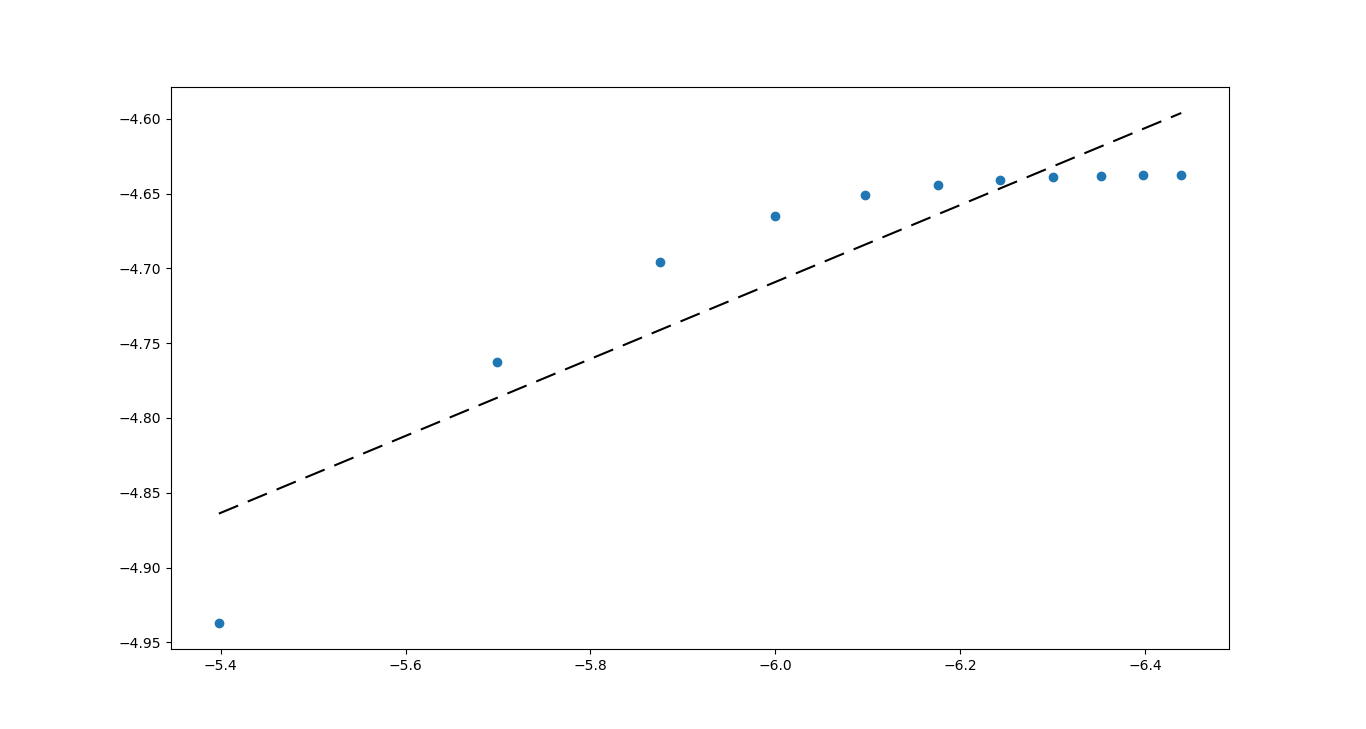
\includegraphics[width=\linewidth]{log-distance.png}
  \caption{A log-log plot of distance $(d)$ from largest timestep collision vs iteratively halving $\Delta$t.}
  \label{Fig 1:}
\end{figure}

Modelling physical phenomena with a discrete timestep ($\Delta t$) carries limitations which a continuous reality (or ideal mathematical system) doesn't; a discrete timestep means we're only simulating part of the 'real' thing. In this instance, we aren't able to pin-point the 'exact' moment that a pair of particles collides. This has two implications: 1) we can't be truly certain of the moment when our (two) final particles collide, and, 2) any prior collisions also suffer the same approximation and have a knock-on effect on our future (final) collision.

It stands to reason that using a smaller $\Delta t$ in our simulation allows us to more accurately approximate either of the two aforementioned scenarios. As we decrease the ($\Delta t$) for our simulation we appear to obtain a more accurate value for the position of the final body.

This hypothesis is supported by the results shown in Fig 1. As $\Delta t \rightarrow 0$, we find that $f(\Delta t$) - the distance between this $\Delta t$'s collision and the largest $\Delta t$ collision - increases, but also appears to converge. $f(\Delta t)$ oscillates around a line of best fit, increasing as we approach the true (real) position of our collision (and hence get further away from the incorrect value).

The most important thing however, is the convergence. This shows what our position does indeed approach a more accurate value as our $\Delta t$ decreases.

\section*{Convergence Order Derivation}

\begin{figure}
  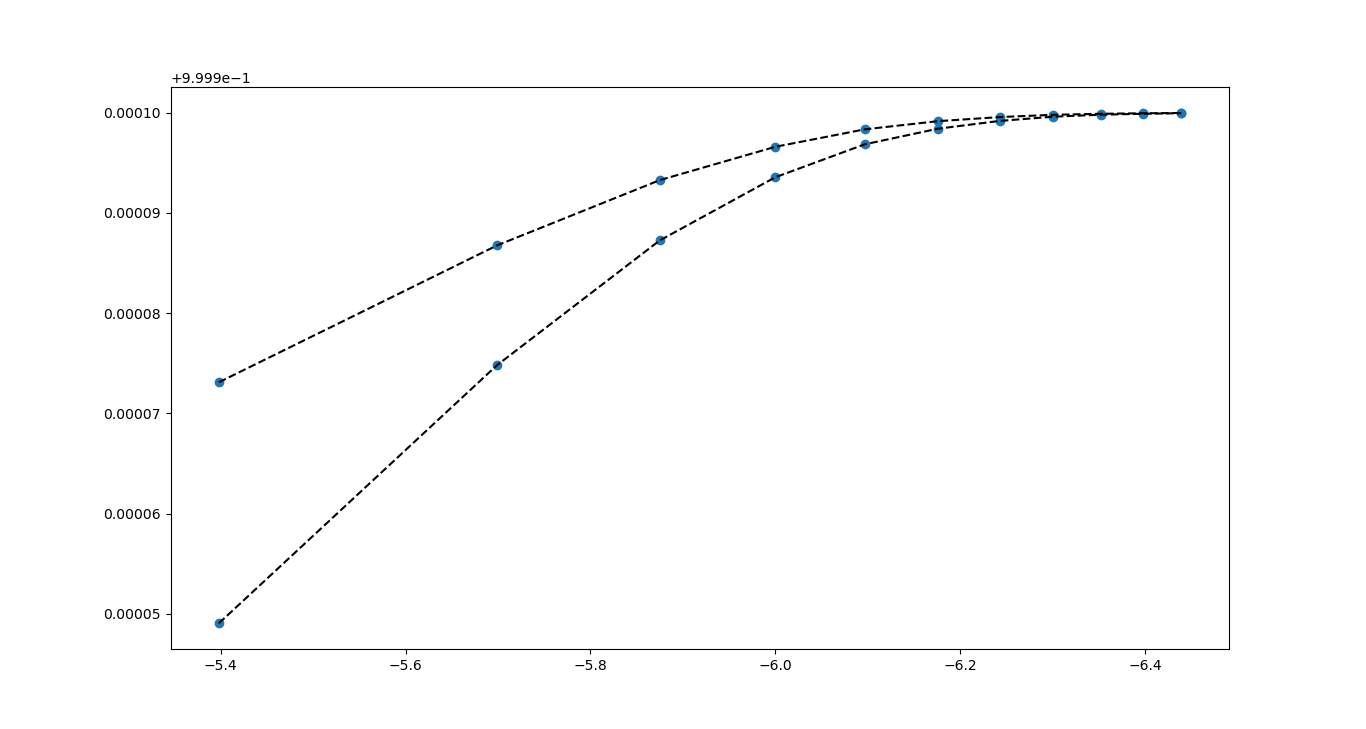
\includegraphics[width=\linewidth]{convergence.png}
  \caption{The value of our limit (for x and y dimensions) for iteratively halving $\Delta$t.}
  \label{Fig 2:}
\end{figure}

\centering
The general form of convergence is:
$$ \lim_{n\rightarrow\infty}{\Bigl|\frac{x_{n+1}-x^*}{x_n-x^*}\Bigr|} = \mu$$
\justifying
To make this form suitable for us, imagine that we have a function mapping $n$ to values of $\Delta t$. Such a function might look like this: $f(n) = \frac{\Delta t}{2^n}$, the power of 2 is used  to relate back to the way in which $\Delta t$ is iteratively halved in the experiment. This now allows us to state that as $n\rightarrow\infty$, $\Delta t\rightarrow0$. Additionally, we can indentify our values of $x^*$ (the true value) as $\{2,1\}$ for dimensions $\{x,y\}$ respectively.

Now: if we consider our experimental calculation (discrete timestep), we can think of $n$ as an array of values $[\Delta t, \frac{\Delta t}{2}, \frac{\Delta t}{4}, \frac{\Delta t}{8}, ...]$ under our function $f(n)$. Our value of $x_n$ is the position of our final collision for some discrete $n$. We know that as $n\rightarrow\infty$, $\Delta t\rightarrow0$, and we (ideally) expect our $x_n\rightarrow x^*$ as $n\rightarrow\infty$.

Fig 2 is plotted for both dimensions $\{x,y\}$, we can see that experimentally, the value of our limit approaches some value $\mu\in(0,1)\oplus(0,1]$. It is not possible to pick which set $\mu$ lies in, in other words, we cannot conclude (experimentally) whether the value ever touches 1. If the value of $\mu=1$ then the convergence is sublinear, but if $\mu<1$ the convergence is linear. We can't deduce this answer without simulating $\infty$ steps.
  
\end{document}
